% 
% ======================================================================
\RequirePackage{docswitch}
% \flag is set by the user, through the makefile:
%    make note
%    make apj
% etc.
\setjournal{\flag}

\documentclass[\docopts]{\docclass}

% You could also define the document class directly
%\documentclass[]{emulateapj}

% Custom commands from LSST DESC, see texmf/styles/lsstdesc_macros.sty
\usepackage{lsstdesc_macros}
\usepackage[utf8]{inputenc}
\usepackage{graphicx}
\graphicspath{{./}{./figures/}}
\bibliographystyle{apj}

% Add your own macros here:



% 
% ======================================================================

\begin{document}

\title{ StarDICE run 3: simulation and performance forecasts }

\maketitlepre

\begin{abstract}
  We describe a model of the expected StarDICE data that is used to
  produce simulated datasets. We then describe the current status of
  the reduction and analysis chain and process simulated data through
  this chain. This draws a forecast of the performance of the next
  campaign as a function of the number of nights and variability of
  atmospheric parameters.
\end{abstract}

% Keywords are ignored in the LSST DESC Note style:
\dockeys{photometry: calibration}

\maketitlepost

% ----------------------------------------------------------------------
% 

\section{Introduction}
\label{sec:intro}

For an isolated point source:
\begin{equation}
  \begin{split}
    \phi_i & \sim \mathcal{P}\left(\tau_\text{exp} \int_{\lambda} d\lambda R(i, \lambda, t) \left[B_i(\lambda) + A(\lambda, t) S(\lambda)\int_{p_i} dx \psi(x - x_0)\right] \right)\\
    \Phi & = \sum_{i \in {Aperture}} w_i \frac1{G(t)} \phi_i + n_i  \quad \text{with } n_i = \mathcal{N}(b_i(t), \sigma_r^2) 
\end{split}
\end{equation}


% ----------------------------------------------------------------------
\section{Components of the photometric response model}
\label{sec:model}

\subsection{Instrumental response}
\label{sec:instrument}

\subsubsection{Detector quantum efficiency }
\label{sec:qe}
We compute the detector quantum efficiency using our NIST calibrated
photodiode (\COMMENT{p-e un lien vers l'Hamamatsu}). Our 24
sharp-spectrum LEDs are put in one side of our photometric test bench
and our camera and the NIST photodiode are placed on the other
side. The detector quantum efficiency beeing the number of electrons
produced when a given photon hit the camera, on one side the number of
photons reaching the photodiode each second can be expressed as:
\[
  N_\text{phot}(\lambda)= \varphi_\text{NIST} \times \frac{\lambda}{hc}
  \frac{1}{\eta(\lambda)}
\]
where $\varphi_{NIST}$ is the flux measured by the NIST in $A$ and
$\eta(\lambda)$ is the NIST quantum efficiency in $A/W$. On the other
side we can express the number of electrons per second that have been
produced in the CCD as:
\[
  N_{e^-} = G \times \varphi_\text{camera} \frac{1}{T_{exp}}
\]
where $G$ is the gain of the electronics in $e^-/ADU$,
$\varphi_{camera}$ the charge accumulated in the CCD and $T_{exp}$ the
time during which the image has been integrated. The idea of this
setup is to use the fact that we have 24 sharp spectrum LEDs from
near-UV to near-IR to get a well-sampled quantum efficiency of our
camera knowing precisely the quantum efficiency of the photodiode and
the SED of our LEDs. We compute the ratio $N_{e^-}/N_\text{phot}$ for
each LED taking into account the geometrical differencies between the
two detectors. The results are shown in Figure \ref{fig:camera_qe}. We
are also currently trying to improve the sampling of the quantum
efficiency by putting a monochromator between the sources and the
detectors which would allow us to select a much smaller wavelength
range of 1nm. But monochromators are coplex objects and the flux that
will be measured depends a lot on the beam incoming on the slit. We
notice some discontinuities for the moment between the measurements
done using different LEDs (and so diffferent positions of the LED beam
according to the slit). We stay for this work with quantum efficiency
we fitst computed.

\begin{figure}[ht]
  \centering
  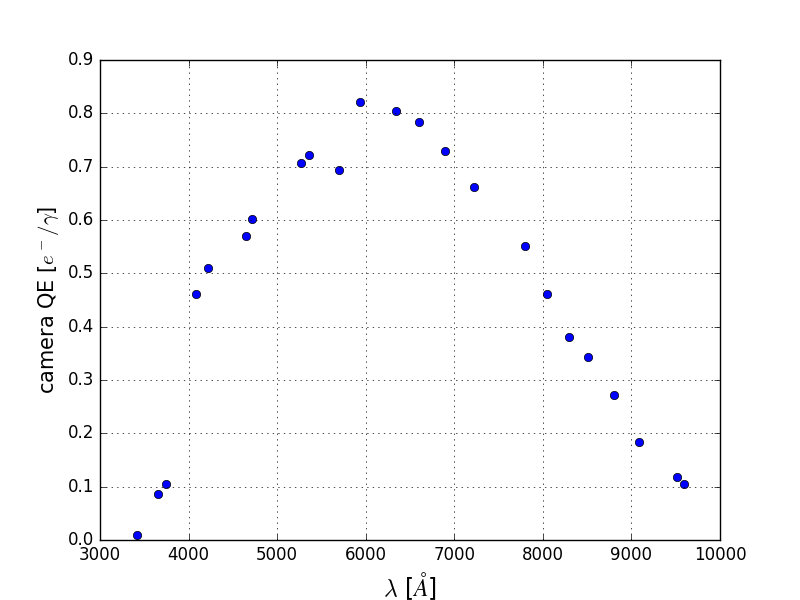
\includegraphics[width=0.7\linewidth]{camera_qe.png}
  \caption{Quantum efficiency in $e^-/\gamma$ of the camera. Each of
    the 23 points represents a measurement of one SnDICE2 LED. We can
    see that it starts to be weak for wavelengths below 400nm and
    above 900 nm.}
  \label{fig:camera_qe}
\end{figure}


\subsubsection{Filter transmission}
\label{sec:filters}
The camera we will use for this third run is equipped of a 5-slots
filter wheel. As an additionnal part of the optics we computed the
transmision of a set of 8 filters by putting back the camera and the
LEDs over the test bench plus putting between a monochromator because
some filters in the set are interferencial filters and thus have sharp
borders that have to be controlled precisely. We put the camera at a
distance where the entire image produced by the monochromator is
included in the CCD. We insert in the filter wheel four filters we
want to chracterize and we let a slot free, then we measure
successively the flux going out from the monochromator with the filter
wheel in each position (including the "free slot" one). We calculate
the transmission of a given filter at a given wavelength as the ratio
between the flux of the LED at the given wavelength selected using the
monochromator in the given filter and the same flux passing through
the empty slot. For each LEDs we insure to select a wavelength that is
inside its spectrum, that allows some "confirmation points" at some
wavelength for which the measurement has been made for 2 different
LEDs and shows no significative difference. The transmission of the 8
filters set is shown in Figure \ref{fig:filters_transmissions}.

\begin{figure}[ht]
  \centering
  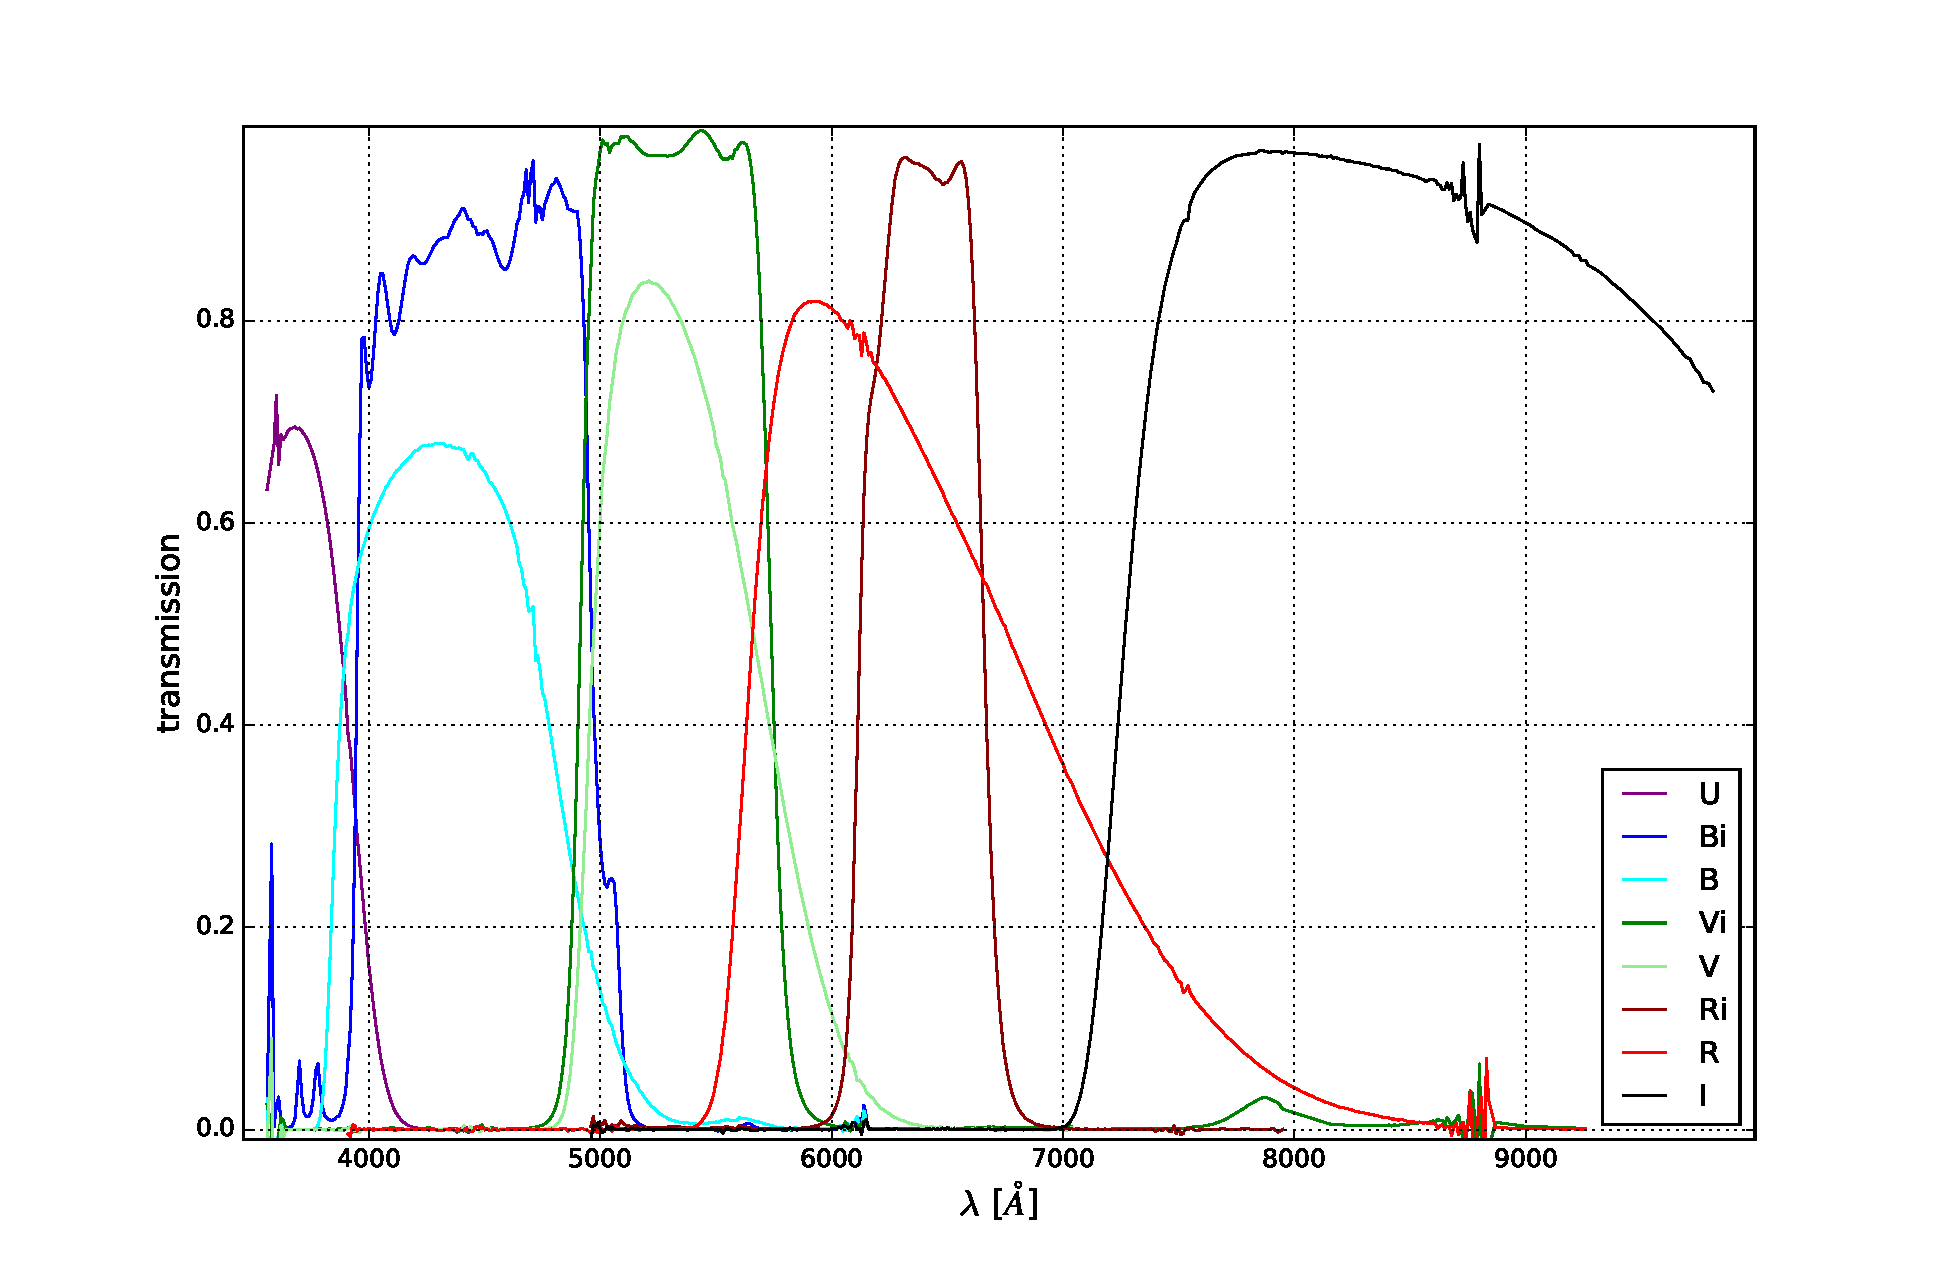
\includegraphics[width=0.7\linewidth]{filters_transmissions.pdf}
  \caption{Transmission of the set of 8 filters at a 1nm
    sampling. Some areas have noisy curves around 870nm and in the UV:
    It is due to a 0 by 0 ratio for the LEDs emmiting very low
    currents at these particular wavelengths.}
  \label{fig:filters_transmissions}
\end{figure}


\subsubsection{Transmission of the optics}
\label{sec:optics}
\COMMENT{Bertrand}

\subsubsection{Instrumental PSF}
\label{sec:PSF}
\COMMENT{Marc,Sylvie,Bertrand}
\begin{itemize}
\item Définition Surfaces
\item Optique polynomiale / zeemacs
\end{itemize}


%------------------------------------------------------------------------------------------------------------------------------------------
\subsection{Atmospherique transmission}
\label{sec:atmosphere}


\subsubsection{Thermodynamical properties of the atmosphere}

\paragraph{Isothermal atmosphere}
\begin{eqnarray}
\frac{dP(h)}{dz} & = & - \rho(h) \cdot g  \nonumber \\
\rho(h)              & = & \frac{M}{RT_0}\cdot P(h) \nonumber \\
P(h)                  &=& P_0 \exp(- \frac{gM}{RT_0}h) \nonumber  
\end{eqnarray}

\begin{itemize}
\item $P_0= $101325 Pa,
\item $T_0=$288.15 K (see level)
\item  $g=$9.80665~m/s$^2$
\item  $M=$0.0289644 kg/mol molar mass of dry air,
\item  $R=$8.31447~J/(mol.K) : universal gas constant). 
\end{itemize}


\subsubsection{Verticall line of sight}
\label{sec:vline}


\subsubsection{Horizontal line of sight}
\label{sec:hline}

\COMMENT{Sylvie et Séb}

%---------------------------------------------------------------------------------------------------------------------------------------
\subsubsection{Stellar line of sight}
\label{sec:av}

\COMMENT{Sylvie et Séb}

\section{Light sources}
\label{sec:sources}

\subsection{LEDs}
\label{sec:leds}
As mentionned earlier, we choose to use LEDs as laboratory calibrated
light sources because of their stability and the ease of their
modelization. The SnDICE2 LED head is composed of 24 sharp spectrum of
$\approx 7\% \lambda_\text{peak}$ width, regulary spread from near-UV to
near-IR. This device was originally designed to produce flatfield
images for MegaCam. This purpose required the LEDs to be supplied with
10 mA, but the current purpose implies to simulate mag 6-7 stars with
this LEDs placed at $\approx 100 m$ from the detector. This requires
the LEDs to be more than $10^4$ times fainter. This also implies the
source to be characterized once again using the spectro-photometric
test bench. Its characterization is divided in two different parts:
the study of the beam produced by the LEDs and the computation of its
spectro-photometric model.

\subsubsection{Beam study}
\label{sec:beam_study}
The study of the beam produced by each LED has already been done in
(((((Regnault et Al 2015)))))\cite{2015A&A...581A..45R,} but we had to
verify that the results obtained are still accurate. In order to study
the beam we produce beam maps by putting the source on our photometric
test bench in front of the NIST photodiode, then at three different
position according the axis of the beam ($d=1300mm$, $d=1800mm $ and
$d=2300mm$) we scan the plan that is perpendicular to the beam axis
every 5mm in $x$ and $y$ (example Figure \ref{fig:beam_map}). The
results we obtain show no major differencies with the previous
one. The beam is homogenous at the percent level with a bump at the
center of the plateau, probably due to some reflexions over the first
mask in the LED head because we see
no non-projective features. \\
Concerning the structure of the beam that we observe, whereas it
wasn't an issue for MegaCam purpose it has to be accounted for the
StarDICE experiment because of our accuracy priors and because when
the source is on site we will get only a small part of the beam. Thus
we have to know precisely where we are in the beam and precisely know
the flux at this particular angle in the beam. Because of the size of
our photodiode ($1cm \times 1cm$) which prevents us from sampling the
beam precisely, we are currently thinking to a setup using a camera to
precisely and quickly map the beam.

\begin{figure}[ht]
  \centering
  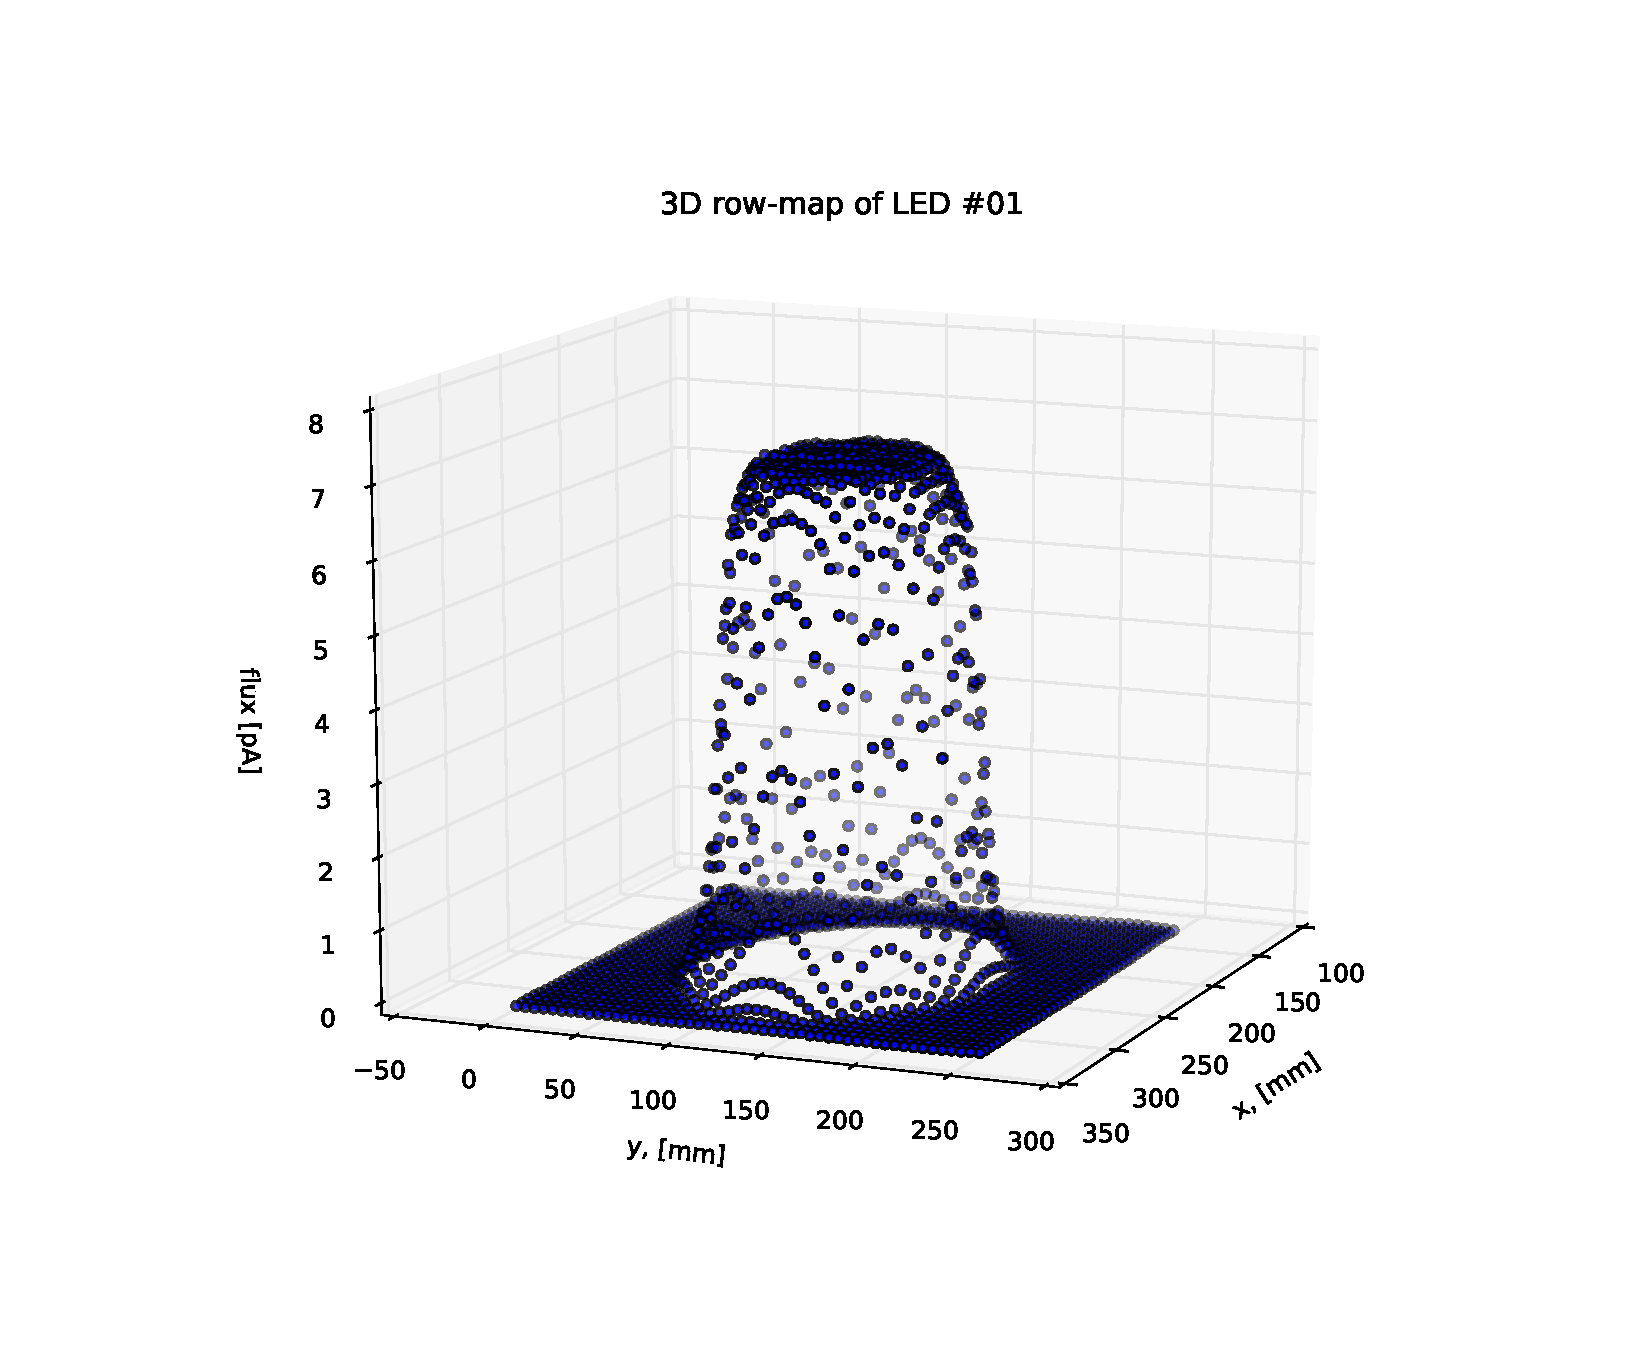
\includegraphics[width=0.45\linewidth]{led-01_3d-map.pdf}
  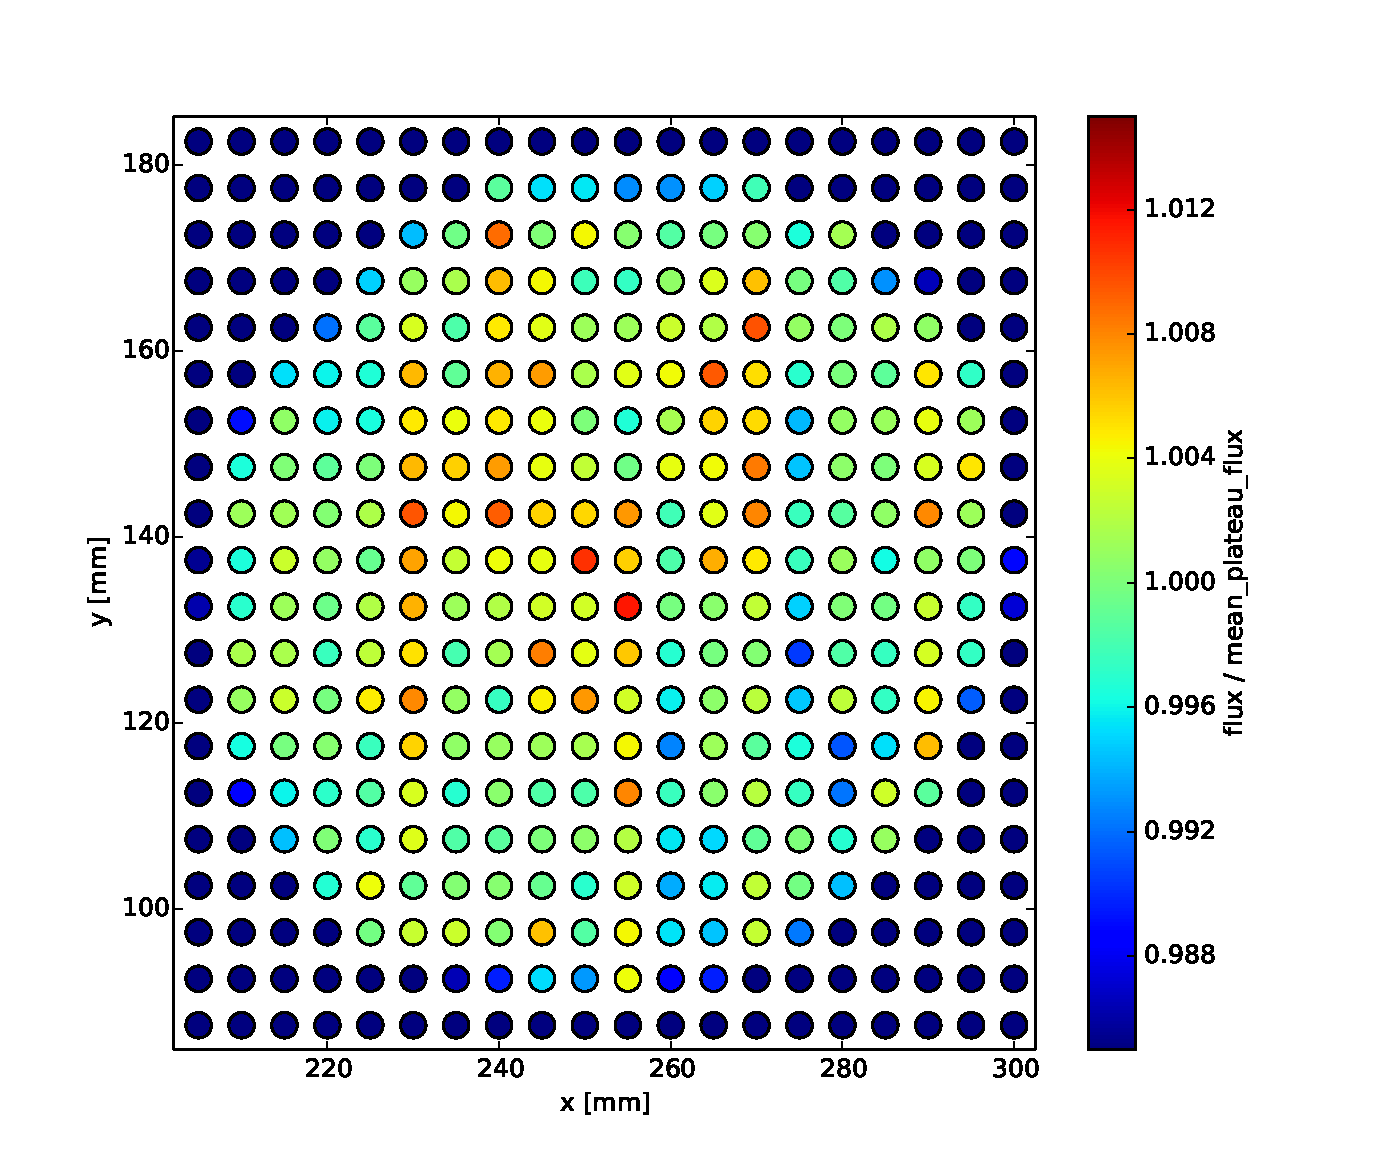
\includegraphics[width=0.45\linewidth]{led-01_plateau-map.pdf}
  \caption{LED \# 01 beam map. Left : Global overview - Right : zoom
    on the plateau of the beam. We see variations at the percent order
    with a structure in the middle of the beam.}
  \label{fig:beam_map}
\end{figure}


\subsubsection{Spectrophotometric Model}
\label{sec:spectromodel}
Our purpose here is to produce a smooth model of the LED spectral
intensities as a function of wavelength in a range of temperatures
that we are likely to have on site at the Observatoire de Haute
Provence. We develop this model on the basis of two-dimensionnal
B-splines:
\[
  S(\lambda, T) = \sum_i \theta_iB_i(\lambda, T)
\]
% where the $\B_i(\lambda, T)$ functions are two-dimensional splines of
% order 3 for the wavelength and order 2 for the temperature, we use one
% node placed approximately every $2 nm$ and one node at each side of
% our temperature dataset range. To constrain we use in a first time
% spectra that we measured on the bench. These spectra are obtained by
% interposing our monochromator between the LED head and our NIST
% photodiode and we scan the flux at each $nm$ over a $\approx 100 nm$
% range. We iterate the measurements at different temperatures regularly
% sampled over the temperature range we already presented. (DIRE CE
% QU'ON COMPTE FAIRE AU NIVEAU DES TEMPERATURES). We modelized each
% measurement of these spectra $\varphi(\lambda, T)$ as follows:
\[
  \varphi(\lambda, T) = \eta(\lambda) \times M(\lambda) \times \sum_i \theta_i B_i(\lambda, T)
\]
where $\eta(\lambda)$ is the quantum efficiency of the NIST photodiode
and $M(\lambda)$ is the relative transmission of the
monochromator. But as we said in \ref{sec:qe}, the absolute
transmission of the monochromator is difficult to obtain and depends
on each spectrum, thus we decided to add this as a nuisance parameter
for each spectra "$f_s$". So the previous equation becomes:
\[
  \varphi_s(\lambda, T) = f_s \times \eta(\lambda) \times M(\lambda)
  \times \sum_i \theta_i B_i(\lambda, T)
\]
In this model, we can see that the normalization of the spectrum is
not constrained because of the degeneracy between the $p_i$'s and the
$f_s$'s. We can break this degeneracy by requiring the normalization
to be fit by our photometric measurements. It is done by adding the
following equation to the model:
\[
  \varPhi(T) = \int_{\lambda} \eta(\lambda) \times
  \sum_i\theta_iB_i(\lambda, T) \quad d\lambda
\]
where $\varPhi(T)$ is the flux measured by the NIST without the
monochromator.\\
The LED spectral intensities are obtained by fitting the model above.

\subsubsection{Results}
\label{sec:leds_results}

\subsection{Stars}
\label{sec:stars}

\COMMENT{Marc}

\subsection{Background light}
\label{sec:background}

\COMMENT{Sylvie, Bertrand, Séb}

\section{Observation plan}
\label{sec:plan}

\subsection{Dataset for the pointing model}
\label{sec:pointingmodel}

\subsection{Dataset for the focus model}
\label{sec:focusmodel}

\subsection{Flatfields}
\label{sec:flatfields}

\subsubsection{Descpription of the dataset and its analysis}
\begin{figure}[ht]
  \centering
  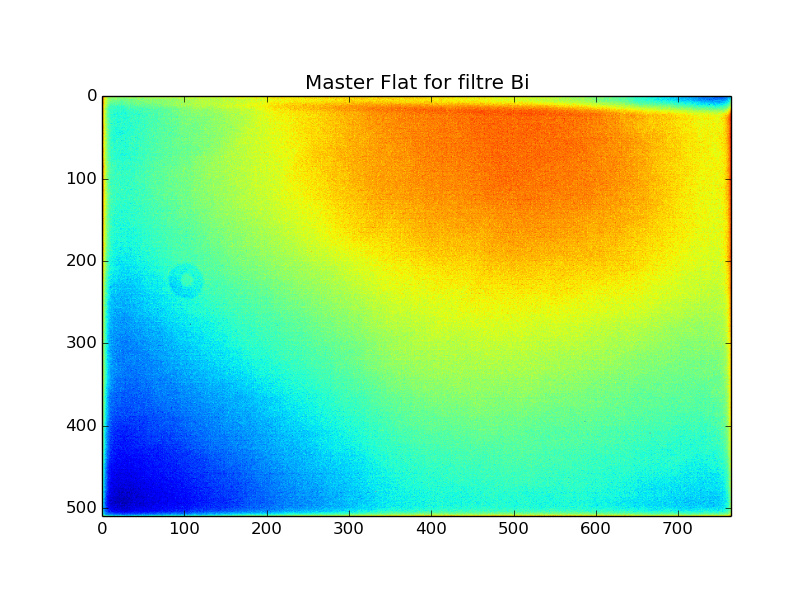
\includegraphics[width=0.45\linewidth]{master_flat_Bi.png}
  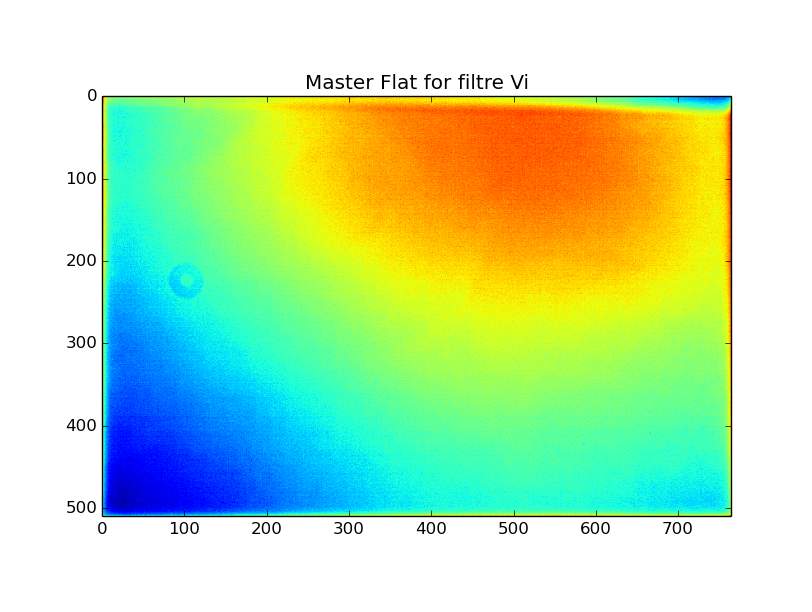
\includegraphics[width=0.45\linewidth]{master_flat_Vi.png}
  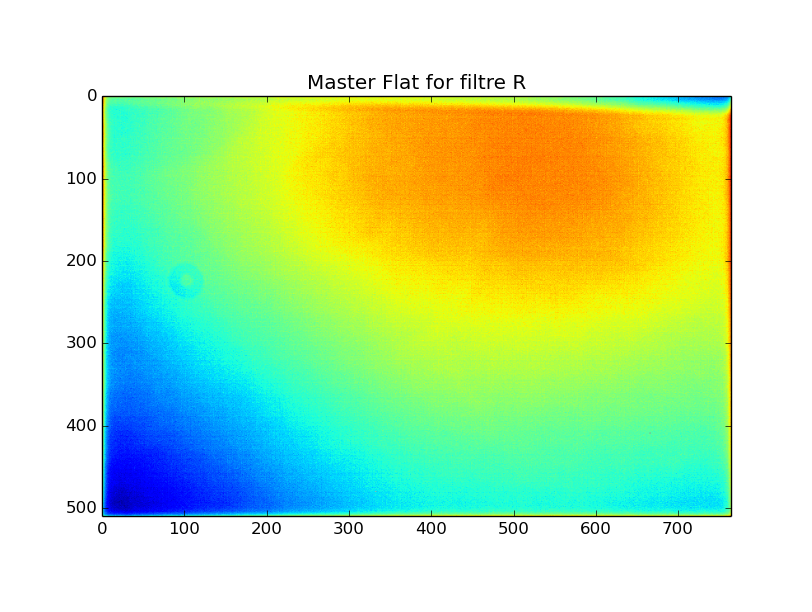
\includegraphics[width=0.45\linewidth]{master_flat_R.png}
  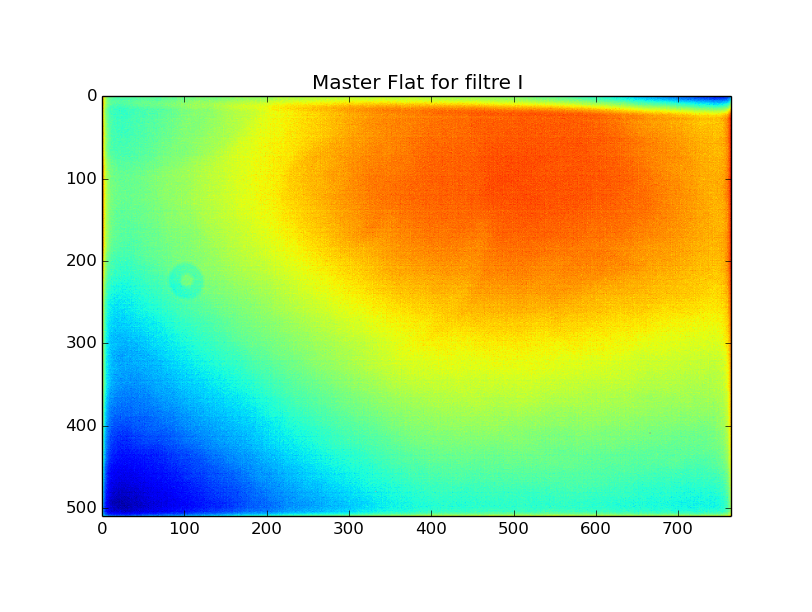
\includegraphics[width=0.45\linewidth]{master_flat_I.png}
  \caption{Master flats for filter $Bi$ (up-left) and $Vi$ (up-right), $R$ (down-left) and $I$ (down-right)}
  \label{fig:master_flats}
\end{figure}

During the second run, the 7th June 2016 we took 231 images of the
twilight sky between 3 and 4 am with 5 different filters (GRISM,
$B_i$, $V_i$, $R$, $I$) and for different exposure times in which we
suppose the flux to be homogeneous. Important deviations from this
model are caused by bright stars and planes going through images
during the exposure. We mitigate the effect of those moving objects by
building a master flat field from successive exposures by an iterative
rejection procedure.

In detail the flux measured in a pixel $i$ of an image $j$ for each
filter is described by the following model of Poisson distribution:
$f_{i,j} = K_jF_i + n_{i,j}$ where $F_i$ is the map of the quantum
efficiency differences common to all images ($<F_i>_i = 1$), $K_j =
<f_{i, j}>_i$ is the global image flux and depends on each image, and
$n_{i, j} \approx N(0, \frac{1}{G}f_{i, j})$.  We want to obtain $F_i$
in order to create a flat field of every image we have for a given
filter.  A solution to the previous model is : $F_i =
\frac{\sum_jK_j}{\sum_j \frac{K_j^2}{f_{i, j}}}$.

But as it has been said previously, some $f_{i, j}$'s should not be
part of our analysis.  The iterative rejection procedure is as follows
:
\begin{itemize}
\item We caluculate $F_i$
\item We mask $(i, j)$ couples for which $|f_{i, j} - K_jF_i| > 5\sigma$
\item We compute again $F_i$ but with the masked dataset
\item We continue until the mask doesn't change from one iteration to another.
\end{itemize}
We notice that ~100 images in the $B_i$ filter can not be used because
we see in them a gradient we don't see in others. The source of this
problem still has to be determined.  But we obtained a master flat
field for each of $B_i$, $V_i$, $R$, and $I$ filters (Figure
\ref{fig:master_flats}).

\subsubsection{Validation of the analysis}
In each band, we take an image of the twilight, we flat field it using
the flat field previously computed and we compare both of them.  As we
can see in Figures \ref{fig:twilight_image_f_3},
\ref{fig:twilight_image_f_2}, \ref{fig:twilight_image_f_4} and
\ref{fig:twilight_image_f_5} except for the objects passing through
the focal plane, the flatfielded images are flat: the shape that was
present in the raw image disappeared. We also notice that the shape of
the different flatfields are quite similar.

\begin{figure}
\centering
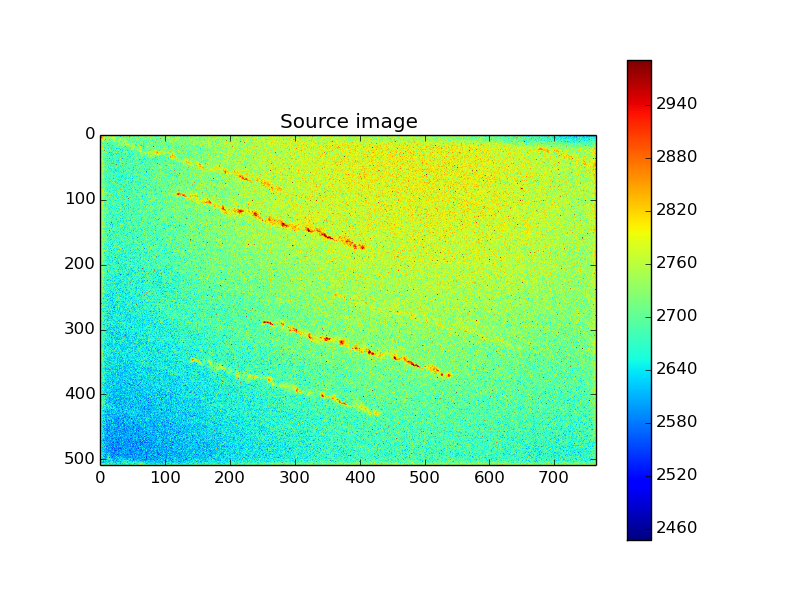
\includegraphics[width=0.45\linewidth]{source_image_filter=3_t=50.png}
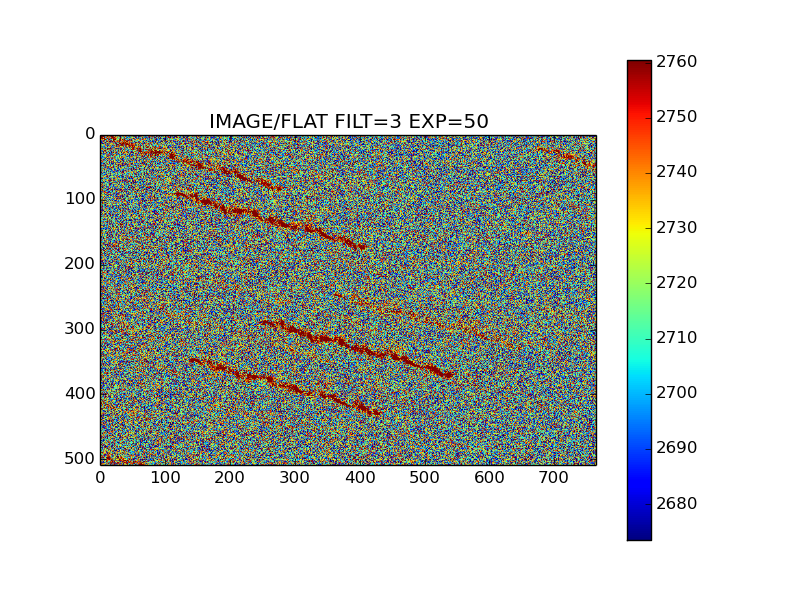
\includegraphics[width=0.45\linewidth]{comp_flat_image_filter=3_t=50.png}
\caption{Left: Twilight image in Vi filter for 50s of exposure. Right:
  Same image divided by the master flatfield. }
\label{fig:twilight_image_f_3}
\end{figure}

\begin{figure}
\centering
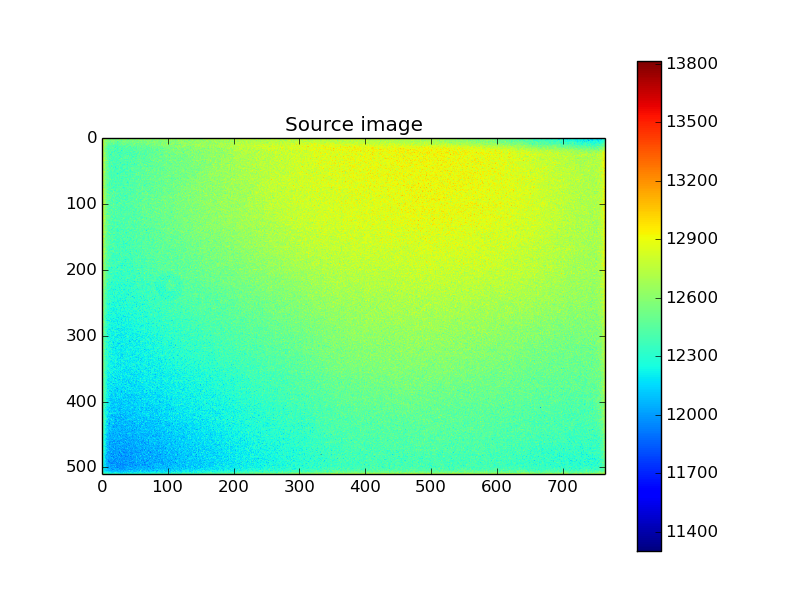
\includegraphics[width=0.45\linewidth]{source_image_filter=2_t=1.png}
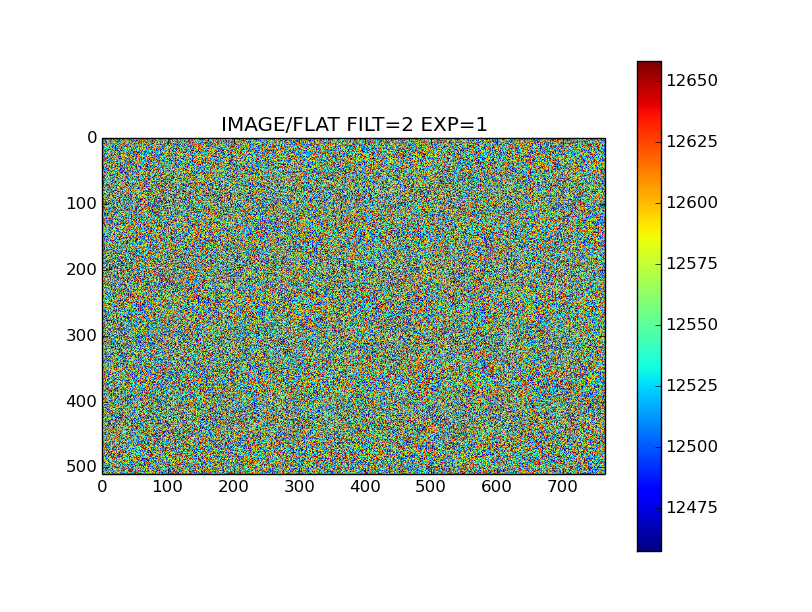
\includegraphics[width=0.45\linewidth]{comp_flat_image_filter=2_t=1.png}
\caption{Left: Twilight image in Bi filter for 1s of exposure. Right:
  Same image divided by the master flatfield. }
\label{fig:twilight_image_f_2}
\end{figure}

\begin{figure}
\centering
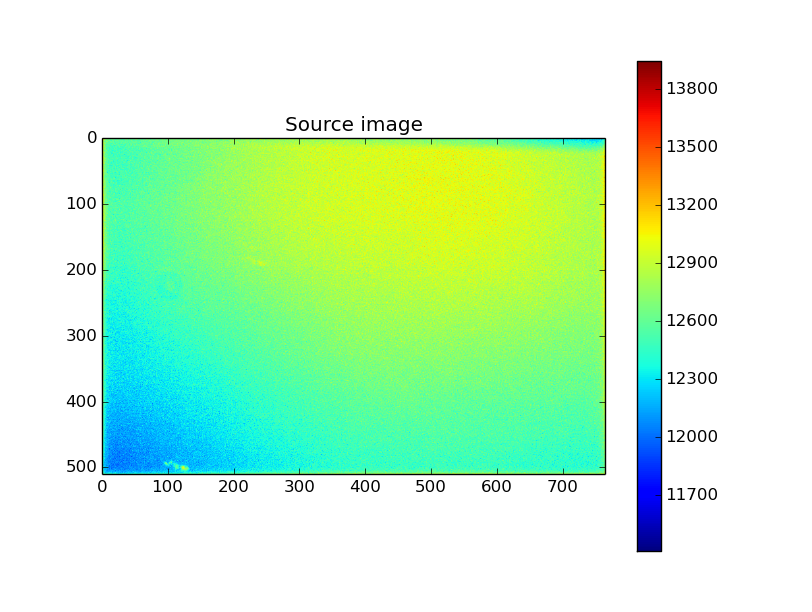
\includegraphics[width=0.45\linewidth]{source_image_filter=4_t=5.png}
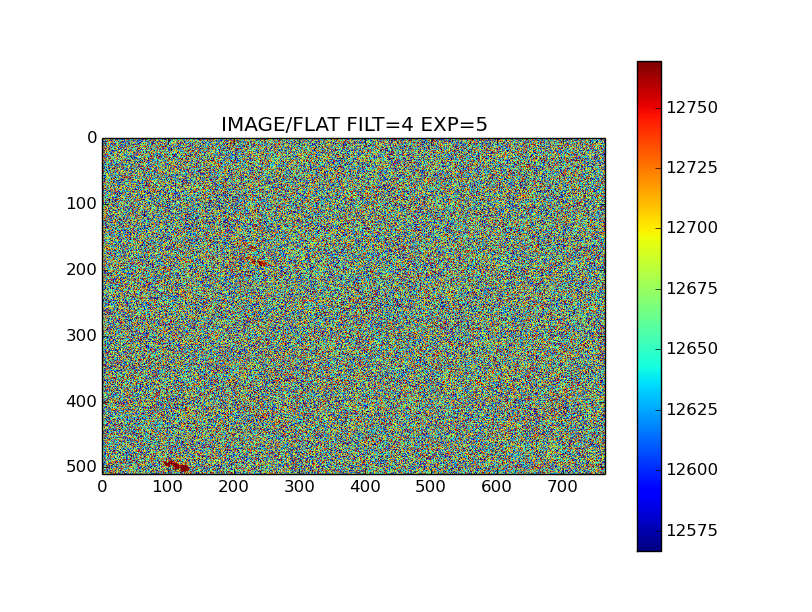
\includegraphics[width=0.45\linewidth]{comp_flat_image_filter=4_t=5.png}
\caption{Left: Twilight image in R filter for 5s of exposure. Right:
  Same image divided by the master flatfield. }
\label{fig:twilight_image_f_4}
\end{figure}

\begin{figure}
\centering
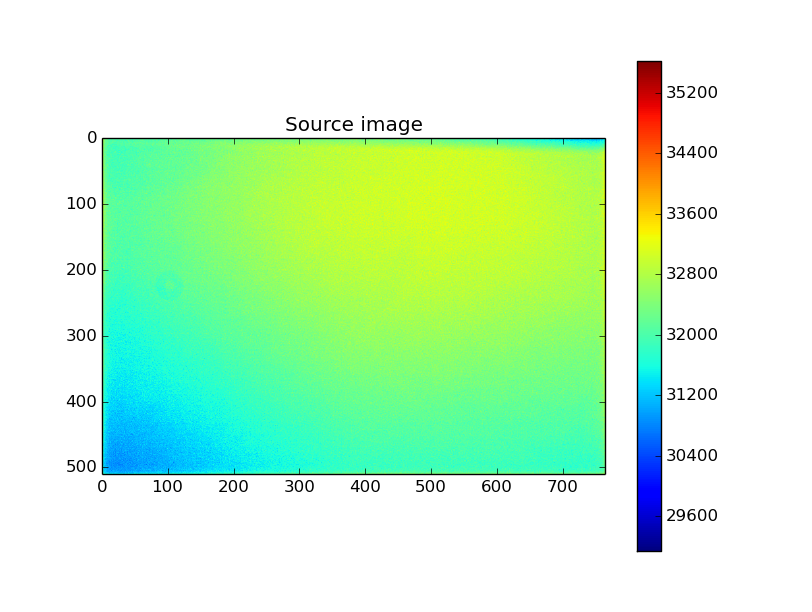
\includegraphics[width=0.45\linewidth]{source_image_filter=5_t=5.png}
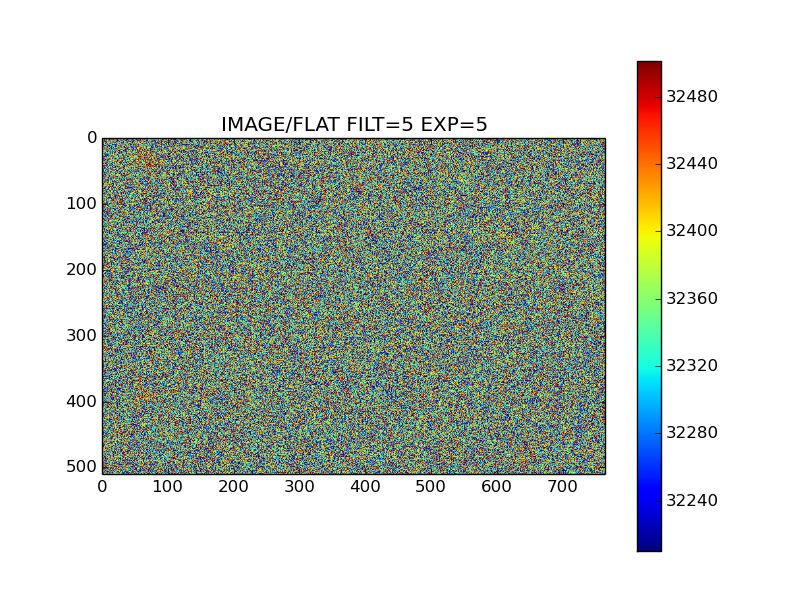
\includegraphics[width=0.45\linewidth]{comp_flat_image_filter=5_t=5.png}
\caption{Left: Twilight image in I filter for 50s of exposure. Right:
  Same image divided by the master flatfield. }
\label{fig:twilight_image_f_5}
\end{figure}

\subsubsection{Photon noise}
\label{subsec:photon_noise}
Using the same statistics we computed the photon noise maps for each
filter (see Figure \ref{fig:photon_noise}) the average photon noise
per pixel : it is on the order of 0.1 \% as we can see in Table
\ref{tab:photon_noise}. These photon noises are compatible with the
success of the experiment.
\begin{figure}[ht]
  \centering
  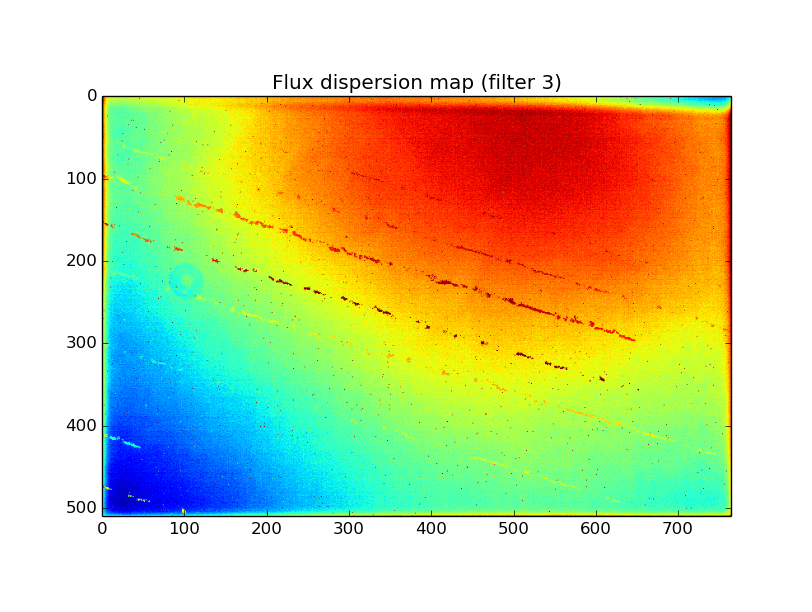
\includegraphics[width=0.90\linewidth]{master_flat_3_var.png}
  \caption{Map of the photon noise : small areas with high photon
    noise are those where we masked data because of objects passing
    through.}
  \label{fig:photon_noise}
\end{figure}

\begin{table}
  \centering
  \caption{Table of the average photon noise in each filter.}
  \begin{tabular}{lccccc}
    \hline
    \hline
    Filter & Bi & Vi & R & I \\
    \hline
    Photon noise / signal (in \%) & 0.185 & 0.118  & 0.101 & 0.073 \\
    \hline
  \end{tabular}

  \label{tab:photon_noise}
\end{table} 

\subsection{Telescopic PSF studies}


\subsection{Science dataset}
\label{sec:data}

\section{Data reduction chain}
\label{sec:dataanalysis}

\COMMENT{Marc et François}
\subsection{Detrending}
\label{sec:detrending}

\subsection{image processing}
\label{sec:processing}

\subsubsection{Source detection}
\label{sec:detection}

\subsubsection{Centroiding}
\label{sec:centroiding}

\subsubsection{photometry}
\label{sec:photometry}

\subsubsection{astrometry}
\label{sec:astrometry}

\subsection{Ancillary data}
\label{sec:ancillary}

\COMMENT{Séb}

\subsection{Catalog analysis}
\label{sec:analysis}


\section{Performance forecast}
\label{sec:forecast}


\section{Conclusion}
\label{sec:conclusion}


\section{Commands}
\label{sec:commands}

There are a number of useful \LaTeX\xspace commands predefined in \code{macros.tex}.
Notice that the section labels are prefixed with \code{sec:} to allow the use of the \verb=\secref= command to reference a section (\ie, \secref{intro}).
Figures can be referenced with the \verb=\figref= command, which assumes that the figure label is prefixed with \code{fig:}.
In \figref{example} we show an example figure.
You'll notice that the actual figure file is found in the \code{figures} directory.
However, because we have specified this directory in our \verb=\graphicspath= we do not need to explicitly specify the path to the image.

The \code{macros.tex} package also contains some conventional scientific units like \angstrom, \GeV, \Msun, etc. and some editorial tools for highlighting \FIXME{issues}, \CHECK{text to be checked}, \COMMENT{comments}, and \NEW{new additions}.


% ----------------------------------------------------------------------

\section{Methods}
\label{sec:methods}

Similar to the figure before, here we have included a table of data from \code{tables/table.tex}.
Notice that again we are able to reference \tabref{example} with the \verb=\tabref= command using the \code{tab:} prefix.
Also notice that we haven't needed to specify the full path to the table because in the \code{Makefile} we include \code{./tables} directory in the \code{\$TEXINPUTS} environment variable.

\begin{table}
  \begin{center}
  \caption{Example table. \label{tab:example}}
  %\begin{ruledtabular}
  \begin{tabular}{lccc}
\hline\hline
Column 1 & Column 2 & Column 3 &  Column 4 \\[3pt]  
     &    $\deg$     & $\kpc$   &  $\deg$ \\[4pt]
\hline
Obj1 & (0,0) & 10 & 0.1 \\
... & ... & ... & ... \\
ObjN & (0,0) & 10 & 0.1
\\\hline\hline
\end{tabular}
\end{center}
%\end{ruledtabular}
\end{table}

%\begin{\tabletype}{l ccccccc }
%\tablewidth{0pt}
%\tabletypesize{\tiny}
%\tablecaption{ An example table. \label{tab:example}}
%\tablehead{
%(1) & (2) & (3) & (4) & (5) & (6) & (7) & (8)\\
%Name & GLON,GLAT & Distance & $r_{1/2}$ & $\log_{10}(J_{\rm meas})$ & $\log_{10}(J_{\rm pred})$ & Sample & Refrence \\
% & (deg) & (kpc) & (pc) & $\log_{10}(\GeV^2 \cm^{-5})$ & $\log_{10}(\GeV^2 \cm^{-5})$ & & 
%}
%\startdata
%Bootes I                     & 358.08,69.62   & 66  & 189  & $18.8 \pm 0.2$ & 18.5           & I,S,C & ... \\
%\\
%...\\
%\\
%Willman 1                    & 158.58,56.78   & 38  & 19   & $19.1 \pm 0.3$ & 18.9           & I,S & ... \\
%\enddata
%{\footnotesize \tablecomments{ (1) The first column. (2) The second column ...}}
%\end{\tabletype}


Equations appear as follows, and can be referred to as, for example, \eqnref{example} -- just as for tables, we use the \verb=\eqnref= command using the \code{eqn:} prefix.
\begin{equation}
  \label{eqn:example}
  \langle f(k) \rangle = \frac{ \sum_{t=0}^{N}f(t,k) }{N}
\end{equation}


% ----------------------------------------------------------------------

\section{Results}
\label{sec:results}

\figref{example} shows an example figure, referred to with the \verb=\figref= command and the \code{fig:} prefix.

\begin{figure}

\includegraphics[width=0.9\columnwidth]{example.png}
\caption{An example figure: the LSST DESC logo, copied from \code{texmf/logos/desc-logo.png} into \code{figures/example.png}. \label{fig:example}}
\end{figure}


% ----------------------------------------------------------------------

\section{Discussion}
\label{sec:discussion}

If you are planning on committing your paper to GitHub, it's a good idea to write your tex as one sentence per line.
This allows for an easier \code{diff} of changes.
It also makes sense to think of latex as \emph{code}, and sentences as logical statements, occupying one line each.
Each line must ``compile'' in the mind of the reader.


% ----------------------------------------------------------------------

\section{Conclusions}
\label{sec:conclusions}

Here's a summary of what we just reported.

We can draw the following well-organized and neatly-formatted conclusions:
\begin{itemize}
  \item This is important.
  \item We can measure some number with some precision.
  \item This has some implications.
\end{itemize}

Here are some parting thoughts.


% ----------------------------------------------------------------------

\subsection*{Acknowledgments}

Here is where you should add your specific acknowledgments, remembering that some standard thanks will be added via the \code{acknowledgments.tex} and \code{contributions.tex} files.

% 
This is the text imported from \code{acknowledgments.tex}, and will be replaced by some standard LSST DESC boilerplate at some point.
% 


\input{contributions}

%{\it Facilities:} \facility{LSST}

% Include both collaboration papers and external citations:
\bibliography{lsstdesc,main}

\end{document}
% ======================================================================
% 
